\documentclass{article}

\usepackage{url} % Tidy web links
\usepackage{microtype} % 'Improved' typesetting
\usepackage{parskip} % Adds white space between paragraphs
\usepackage[super]{natbib} % Citations using superscript
\usepackage[a4paper, left=2.cm, right=2.0cm, top=2.0cm, bottom=2.0cm]{geometry}
\usepackage{longtable,booktabs}  % For tables
\usepackage{caption} % For figure and table captions
\usepackage{graphicx} % Adds more functionality to graphics for inclusion of figures
\usepackage{lineno} % Allows use of \linenumbers to add line numbers 
\usepackage[toc,page]{appendix}
\usepackage[utf8]{inputenc}
\frenchspacing % No double spacing between sentences
\linespread{1.2} % Set linespace
\usepackage{authblk} % For author formatting
\usepackage{lmodern} % A scalable font - avoids erros due to non-sclabale fonts
\usepackage{subcaption} % Allows use of subfigures
\DeclareUnicodeCharacter{2060}{\nolinebreak} % Prevent unicode (U+2060) error on local complile
\usepackage{cclicenses} % For creative commons license
\usepackage{xcolor} % for coloured text
\usepackage{xurl} %for url but with more flexible linebreaking

\usepackage{markdown}

% Choose your own colour
\usepackage{color}
\newcommand{\mjanote}[2][\textcolor{red}{\dagger}]{\textcolor{red}{$#1$}\marginpar{\color{red}\raggedright\tiny$#1$ #2}}
\newcommand{\mjaFIXME}[1]{\textcolor{red}{[\textbf{FIXME} \textsl{#1}]}}
\newcommand{\kpnote}[2][\textcolor{magenta}{\dagger}]{\textcolor{magenta}{$#1$}\marginpar{\color{magenta}\raggedright\tiny$#1$ #2}}
\newcommand{\kpFIXME}[1]{\textcolor{magenta}{[\textbf{FIXME} \textsl{#1}]}}

\hbadness=1000000 % Turn off \hbox badness warnings

\begin{document}
% Rewrite this title to include dementia

\title{STROKE-FLOW: Using explainable machine learning and clinical pathway simulation to model and optimise flow and capacity planning in the in-patient stroke pathway.}

\author{} % Hide author
\date{} % Hide date
\maketitle
\vspace{-20mm}
\section{Summary}

The focus of our work is on using explainable machine learning and clinical pathway simulation, applied to national clinical audit data to identify between-hospital variation in clinical decision-making, and understanding the impact of that variation on patients and the health service. Our work is in collaboration with the Sentinel National Stroke Audit Programme, and focuses mostly on the emergency stroke pathway, and variation in use of clot-busting drugs (the primary treatment of emergency stroke admissions), but is applicable across other clinical areas.

In the proposed project we would like to bring multiple NIHR project strands together in a single framework, and progress the modelling to include acute and rehab in-patient care. As a result we will be able to evaluate how variation in clinical decision-making and processes effect both the patient and bed requirements for in-patient stroke care. This will allow planners to see how an optimal system may behave in their area (e.g. at the level of integrated stroke delivery teams, or integrated care systems). Analysis and modelling will be made available through a web application.

The project will be a multi-methods study including machine learning, clinical pathway simulation, geographic modelling, and qualitative research. The team has the necessary skills and experience, with a well-established track-record, to undertake this work.

\subsection{Process flow in scope}

The work will focus on out-of-hospital stroke patients who call for an ambulance, the system in scope is shown in figure \ref{fig:flow}.

\begin{figure}[h]
\centering
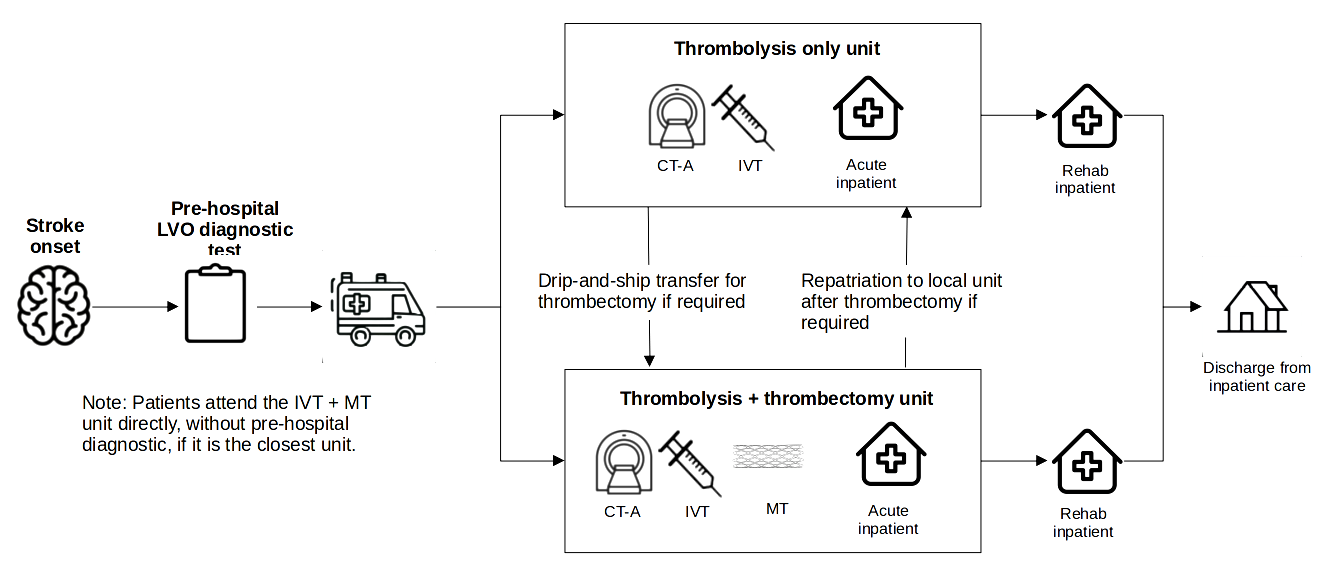
\includegraphics[width=1.0\textwidth]{./images/pathway}
\caption{Summary of patient flow}
\label{fig:flow}
\end{figure}


\subsection{Research questions}

\begin{markdown}
* How much of the variation in required stroke inpatient resources comes from differences in local patient populations, and how much from differences in variation in clinical decision-making and processes?
* How would optimal provision of thrombolysis and thrombectomy (including decision-making on selecting suitable patients) affect outcomes and required stroke inpatient resources?
* How would pre-hospital triage for patients suitable for thrombectomy affect outcomes and required stroke inpatient resources?
* What are hospitals with good outcomes and shorter lengths of stay (after allowing for differences in local populations) doing differently, compared with those with longer lengths of stay?
\end{markdown}


%\section{Bid info}

\url{https://www.nihr.ac.uk/funding/2310-health-and-social-care-delivery-research-programme-researcher-led/32515}

\subsection{Timelines}

\begin{markdown}
* Stage 1 deadline: 1pm, 20 September 2023
* Notification of out of remit/non-competitive decision if unsuccessful: late October 2023
* Notification of Stage 1 shortlisting decision: early December 2023
* Stage 2 writing window: early December 2023 to early February 2024
* Notification of Stage 2 funding decision: early April 2024
* Start date for funded studies: 1 August/September 2024
\end{markdown}
%\begin{markdown}
# Background

## Process flow in scope

* Onset to ambulance call
* Ambulance response
* Pre-hopsital triage
* Acute care:
    * Reperfusion treatment (thrombolysis and thrombectomy)
    * Transfer/repatriation as required
    * Acute care in-patient stay
* In-patient rehab care stay
* Discharge destination


## Related projects

SAMueL-1:
https://fundingawards.nihr.ac.uk/award/17/99/89

SAMueL-2:
https://fundingawards.nihr.ac.uk/award/NIHR134326

OPTIMIST:
https://fundingawards.nihr.ac.uk/award/NIHR202361

MUSTER:
https://fundingawards.nihr.ac.uk/award/NIHR153982    
\end{markdown}



\end{document}